\chapter{Application}\label{Ch.5}
This chapter will utilise methods described in the previous chapters to derive the risk-neutral density for call options on numerous underlying stocks. The risk-neutral density will be estimated by constructing a neural network which estimates the implied volatility, which derivatives will be estimated using finite difference. Afterwards, the risk-neutral density will be used to derive option prices to test the method's performance.

The project's code and data is available on GitHub: \url{https://github.com/loprtq/P8}.


\section*{Data}
As mentioned, we will be working with numerous underlying stocks, specifically: Apple Inc. (AAPL), Amazon Inc. (AMZN), Tesla Inc. (TSLA), and Alphabet Inc. Class C (GOOG). These stocks have been chosen because of their varying liquidity and vast option data. For these stocks we retrieve information about the stock price, option price and the option's strike prices and time to maturities. Additionally, we set the risk-free rate to $r=0.0368$ and calculate the implied volatility according to the method seen in \eqref{Eq:IV_formula} using the function "\lstinline{EuropeanOptionImpliedVolaitlity}". We will first give a detailed description of the application on the stock GOOG followed by a shorter analysis of the other stocks.

Given that we want to work with an implied volatility surface for which all data has the same stock price at the retrieval time, we filter the data with respect to the stock price. For GOOG, this stock price is, as we will see, approximately $S_t=100$, meaning options with stock prices below and above this are removed. Likewise, as we saw in \autoref{Sec.Implied_Volatility}, the volatility smile is more distinct when close to maturity, why we remove time to maturities larger than $0.1$ years (approximately 36 days).

Having filtered the data for GOOG we end up with approximately $11.000$ data points, where the strike price and time to maturity is distributed as seen in \autoref{Figures:Figures/Pictures/KDist.pdf} and \autoref{Figures:Figures/Pictures/TDist.pdf}, respectively. As is evident in \autoref{Figures:Figures/Pictures/KDist.pdf}, most strike prices are around ATM ($100$) with very few points far away. Furthermore, as expected when retrieving the data there are some gaps in time to maturity, which could be due to weekends. Moreover, the time to maturities are fairly spread out over the time period. Because of this, it is expected that when constructing a neural network for the implied volatility surface that it, in general, will be more precise around ATM as a consequence of the distribution of the data. 

\dimgfig{Figures/Pictures/KDist.pdf}{Distribution of strike prices for GOOG after filtering the data.}{Figures/Pictures/TDist.pdf}{Distribution of time to maturity for GOOG after filtering the data.}

When working with the data, we choose to normalise the inputs in the neural network, that is strike price and time to maturity, as this equalises the scale of input features and make it easier for the model to learn, without distorting it - the data keeps its differences and distribution. Additionally, some of the algorithms used to create the neural network performs better when using normalised data, as it, for example, helps the gradients converge to the minimum faster, and makes the network perform better in general.

The reason why strike price and time to maturity are the input variables in the neural network is that these are the variables the implied volatility surface depends on, given a stock price, $S_t$. This can also be seen in \autoref{Figures:Figures/Pictures/Volatility Surface Scatter (GOOG).png}, which is the implied volatility data points for the filtered data where, $S_t = 100$. 

\imgfig[0.5]{Figures/Pictures/Volatility Surface Scatter (GOOG).png}{Implied volatility of GOOG for $S_t=100$.}

In \autoref{Figures:Figures/Pictures/Volatility Surface Scatter (GOOG).png} we see that as we approach maturity, the volatility smile becomes more skewed. Besides this, we observe that there are few points far away from ATM ($100$). Another thing to note is that the points that are further from ATM have higher implied volatility, resembling the theory presented in \autoref{Sec.Implied_Volatility}. All of this can affect the neural network constructed in the next section, and will be further analysed in later sections. 

\section{Neural Network for Implied Volatility}\label{Sec.App:NN}
For the construction of the neural network the package "\lstinline{tensorflow}" is used alongside the "\lstinline{keras}" package. After sorting the data there are, as mentioned, approximately $11.000$ input-output pairs left which should be split into three batches: training-, validation-, and test sets. We have opted to split the data into the three sets, allocating 50\% for training, and 25\% each for validation and testing. This method of splitting the data is widely used, and hence adopted. The validation set is utilised to identify overfitting by contrasting the model's error on the training set with that of the validation set. If the training set's error is below that of the validation set, it may suggest the presence of overfitting. An example of such behavior can be seen in \autoref{Figures:Figures/Pictures/Application/Overfitting_loss_mae.pdf}. Contrarily, if the training set's error is far above that of the validation set, it may suggest the presence of underfitting.

\imgfig[1]{Figures/Pictures/Application/Overfitting_loss_mae.pdf}{MSE, MAE and MAPE on training- and validation set.}

In \autoref{Figures:Figures/Pictures/Application/Overfitting_loss_mae.pdf} it is evident that throughout all $20$ epochs the network performs better on the training set than on the validation set, where the error is measured by the mean squared error (MSE), mean absolute error (MAE), and mean absolute percentage error (MAPE). MSE is chosen as it penalises the larger errors more heavily and is also widely used as loss function in neural networks. MAE is chosen as it gives an indication of the average error. MAPE is chosen because it takes the error's magnitude into account, making the errors easier to interpret.

Another detail about the MAE and MAPE on the validation set is that it has big jumps. These jumps are not desirable as it indicates that the neural network is not learning in a stable and consistent manner. A validation error curve with sudden jumps can further indicate that the neural network is overfitting to the training set. This can, for example, be adjusted by changing the learning rate. 

When constructing the neural network there is not one correct neural network, but choosing one with the smallest MSE, MAE, and MAPE as well as with no overfitting is advisable. Though, one should also take into consideration the reduction in error compared to the increase in parameters. This is because, as the number of parameters increase so does the number of computations, and the computational time.

We start the construction of the neural network by choosing the number of layers followed by the number of nodes in each layer. We have chosen the loss function as the MSE since this is widely used for function approximations. Furthermore, the identity function is chosen as the activation function in the output layer, and a fixed activation function is chosen for the hidden layers. In order to ensure a fair comparison of network performance, we tested networks with a variety of layers and nodes, all trained for a fixed number of $50$ epochs, a minibatch size of $128$ per gradient update, and Relu as the activation function. Specifically, we evaluated networks with one, two, three, and four layers, each with a wide range of nodes. To minimise variability in the experimental setup, we kept the optimiser fixed as the Adam optimiser with a learning rate of $0.001$ and decay rates $0.999$ and $0.9$. Additionally, we used fixed training-, validation-, and test sets, as well as a set seed for each network to ensure reproducibility. Finally, we did not apply any dropout to any of the layers. All of these measures were taken to ensure that any observed differences in performance between the networks were primarily due to their architectural differences, rather than other factors such as differences in training procedures or data set partitioning.

Our comparison revealed that increasing the number of layers led to a significant improvement in both the MSE, MAE, and MAPE, with the greatest improvements observed when transitioning from one to two layers, and from two to three layers. However, when adding a fourth layer, we did not observe a clear improvement in network performance. Moreover, we observed an indication of overfitting as the validation and test errors exceeded that of the training set when adding a fourth layer. A sample of the different networks tested can be seen in \autoref{Table:NN}, where "\# of nodes" describes the number of nodes in each hidden layer. As these tests were difficult to compare, we choose to focus on neural networks where the number of nodes in each hidden layer were equivalent. However, we additionally tested some neural networks with a differing number of nodes in each layer.

\begin{table}[H]
    \centering
    {\renewcommand{\arraystretch}{1.25}\begin{tabular}{c|cccc}
        \# of nodes &  1 layer & 2 layers & 3 layers & 4 layers\\\hline
        5   & 7.5432\% & 7.2432\% & 7.1389\% & 7.1069\% \\ \hline
        20  & 7.1745\% & 5.7547\% & 5.3227\% & 5.3038\% \\ \hline
        60  & 7.0909\% & 5.2964\% & 5.0457\% & 4.9905\% \\ \hline
        110 & 6.2565\% & 5.1217\% & 4.8618\% & 4.8618\% \\ \hline
        210 & 6.1858\% & 5.0628\% & 4.8540\% & 4.8495\%
    \end{tabular}}
    \caption{MAPE for different neural networks all trained with a fixed seed.}
    \label{Table:NN}
\end{table}

As a result, we concluded that a neural network with three hidden layers provided the optimal balance of performance and generalisation ability, and we therefore chose to use this architecture for our subsequent analyses. The preceding analysis was conducted by evaluating up to forty networks for each number of layers, in order to ensure that our conclusions were robust and not based on a limited sample size. 

After choosing the number of layers, we went on to choose the optimal number of nodes in the network. Here we tried fifty combinations of number of nodes from very small networks with two nodes in each layer up to 250 nodes in each layer. Furthermore, we experimented with the shape of the network. That is, if it was better to start with a wide layer and end with a narrow layer, vise versa, or just have the same width throughout all of the layers. We concluded that the neural network with $110$ nodes in each of the three hidden layers was the neural network that performed best without clear indication of overfitting. This performance can also be seen in the fourth column of \autoref{Table:NN}, where the MAPE decreases approximately $0.2$ going $5$ to $20$, $20$ to $60$, and $60$ to $110$ nodes, but only $0.02$ going from 110 to 210 nodes. That means our network has the same architecture as \autoref{Figures:Figures/Neural_networks/3_layer_NN.pdf} in \autoref{Ch.3}, where $K_0=2$, $K_1 = K_2 = K_3 = 110$ and $K_4 = 1$.

After choosing the architecture we experimented with minibatch sizes, activation functions, and other optimisers such as RMSProp, by training multiple different neural networks varying these three things. Within this training we established that a minibatch size of $32$, the Adam optimiser, and the Relu activation function performed the best. Lastly, the optimal combination of dropout-, learning-, and decay rates needs to be determined. However, it is too time-consuming to test all possible combinations of dropout-, learning-, and decay rates manually. Hence, we used the function "\lstinline{tuning_run}" from the package "\lstinline{tfruns}" which runs a hyperparameter tuning experiment based on a given set of parameters to choose among. We chose multiple dropout rates for each hidden layer and multiple learning- and decay rates all seen in \autoref{Table:NN2}. We chose that the function should test 30\% of the possible combinations at random from which we chose the one that performed the best.

\begin{table}[H]
    \centering
    {\renewcommand{\arraystretch}{1.25}\begin{tabular}{c|c}
        dropout rate layer 1  & $\left\{0, 0.2, 0.5 \right\}$\\ \hline
        dropout rate layer 2  &  $\left\{0, 0.2, 0.5\right\}$\\ \hline
        dropout rate layer 3  &  $\left\{0, 0.2, 0.5\right\}$\\ \hline
        learning rate         &  $\left\{0.0001, 0.0005, 0.001\right\}$\\ \hline
        decay rate $\alpha$   &  $\left\{0.9, 0.95, 0.99\right\}$\\ \hline
        decay rate $\alpha_f$ &  $\left\{0.8, 0.85, 0.9\right\}$\\ 
    \end{tabular}}
    \caption{Possible dropout-, learning, and decay rates in "\lstinline{tuning_run}".}
    \label{Table:NN2}
\end{table}

Even though it does not seem as many possible choices, it is a total of 730 different combinations where the function then chooses 219 random combinations. From this there is a clear indication that the neural network performs best when $\alpha_f = 0.8$, $\alpha = 0.9$ and the learning rate is $0.0005$. These results can be found in \url{https://github.com/loprtq/P8/tree/main/Code/Data}. When the other hyperparameters are varied the errors in the validation set is the same or vary close to each other. Hence, we try running these neural networks for a greater number of epochs both to see how the performance changes when training the neural network more, and to see if some or all of the networks have an indication of overfitting. From this we get that the neural network performs best when the dropout rate in the first, second and third layer is $0$, $0$ and $0.2$, respectively. Hence, we have chosen a neural network to work with based on the "\lstinline{tuning_run}" function and manually checking for overfitting. That is, a neural network with two input nodes, one output node and three hidden layers each with 110 nodes, a dropout rate of 20\% in the last hidden layer and decay rates $\alpha = 0.9$ and $\alpha_f = 0.8$. Furthermore, the neural network uses the Relu activation function, has a learning rate of $0.0005$ and a minibatch size of $32$. Lastly, this neural network keeps improving without any indication of overfitting up till $1200$ epochs. Note that we also tried including a learning rate as the exponential decay described in \autoref{Ch.3}, but saw no clear improvement,  why we did not use it.

Furthermore, the MSE, MAE and MAPE is illustrated in \autoref{Figures:Figures/Pictures/Application/errorplot_final.pdf}.
\imgfig[1]{Figures/Pictures/Application/errorplot_final.pdf}{MSE, MAE and MAPE on training- and validation set.}

Here it is seen that there are no clear indication of overfitting in either the MAE, MSE or MAPE plot. Furthermore, there is some variability in the MAE and MAPE of the validation data set. However, these values are so small that they are considered inconsequential. 

After conducting this thorough analysis, we proceed with the data processing using this specific neural network. To further asses the neural network we plot an implied volatility surface constructed by the chosen neural network together with the test data seen in \autoref{Figures:Figures/Pictures/Application/vol_surfaceNN.pdf}. 
\imgfig[1]{Figures/Pictures/Application/vol_surfaceNN.pdf}{Volatility surface from neural network compared with test data set (orange points).}

\autoref{Figures:Figures/Pictures/Application/vol_surfaceNN.pdf} reveals that the implied volatility surface created by the neural network exhibits a volatility smile, which closely resembles the one observed in the data. This is also evident in the MSE, MAE, and MAPE when evaluating the network on the test data set, seen in \autoref{Table:NN3}. Hence, this reinforces the choice of neural network.

\begin{table}[H]
    \centering
    {\renewcommand{\arraystretch}{1.25}\begin{tabular}{c|c}
        MSE  &  0.0002\\ \hline
        MAE  &  0.0089\\ \hline
        MAPE &  2.1075\%\\ 
    \end{tabular}}
    \caption{MSE, MAE and MAPE for the test data set.}
    \label{Table:NN3}
\end{table}

Furthermore, to illustrate the error we plot the real values of the implied volatility against the prediction of the neural network, in a so called prediction plot, which is seen in \autoref{Figures:Figures/Pictures/Application/lineplot.pdf}. For the neural network to perform perfectly, its predictions must follow a diagonal line, illustrated as the black line in \autoref{Figures:Figures/Pictures/Application/lineplot.pdf}. In \autoref{Figures:Figures/Pictures/Application/lineplot.pdf} we see that even though the predictions do not follow the black line exactly, it is close.
\imgfig[1]{Figures/Pictures/Application/lineplot.pdf}{Prediction plot of the neural network estimating the implied volatility surface. The black line is the theoretical best regression whereas the blue line is the achieved regression.}

Furthermore, we have fitted a linear regression to the predictions as a function of the real values, which is illustrated by the blue line in \autoref{Figures:Figures/Pictures/Application/lineplot.pdf}. The linear regression is constructed using the "\lstinline{lm}" function which has an associated "\lstinline{summary}" some of which can be seen in \autoref{tab:summary_af_lm}.
\begin{table}[H]
    \centering
    \begin{tabular}{ccc}
    \hline\addlinespace[1ex]
        \multicolumn{3}{c}{Coefficients}\\
          & Estimate & Std. Error \\
         Intercept & $0.0428$ & $0.0017$ \\
         Real Value & $0.8956$ & $0.0040$ \\
    \addlinespace[1ex]\hline\addlinespace[1ex]
        \multicolumn{3}{c}{$R^2$: $0.9435$, $R^2$ Adjusted: $0.9435$}\\
    \addlinespace[1ex]\hline
    \end{tabular}
    \caption{Summary of the model "\lstinline{lm(Predictions ~ Real Value)}".}
    \label{tab:summary_af_lm}
\end{table}

As described before, the neural network would perform perfectly if the "Estimate" in had the value $1$ for "Real value" and $0$ for "Intercept" implying that $R^2=1$. However, it is seen that both the "Estimate", and the $R^2$ are below one, more precisely $0.895618$ and $0.9435$, respectively. This indicates that the neural network performs fairly well, but there are room for improvement. Further improvements can possibly be found, by again, using "\lstinline{tuning_run}" for an extended set of possible parameters.

Note that, as mentioned, the neural network we have selected may not necessarily be the optimal one, as the process of choosing a suitable architecture is complex and subjective. Additionally, due to time constraints, we were unable to experiment with an extensive amount of neural networks, and approaches. Hence, we acknowledge that our chosen network may have limitations, meaning there can exist a better choice.

Using the neural network we then determine the derivatives of the implied volatility with respect to the strike price once and twice. This is done as described in \autoref{Ch.4} by numerically differentiating the implied volatility using finite difference. When using the finite difference method on the implied volatility we started of by using the first and second order central difference method for calculating the derivatives. As the second order central difference did not perform very well we opted to try using the first order central difference, in \eqref{eq:central_diff}, twice in which case we obtained smoother results. This lead us to choose this methodology over the second order central difference method. 


% \section{Risk-Neutral Density}\label{Sec.App:RND}

% As the terms in \eqref{Eq:RND_Derivatives} have all been estimated, it is now possible to determine the risk-neutral density by rewriting \eqref{Eq:PartialC} to
% \begin{align}\label{Eq:App_RND}
%     \exp\left(r\tau\right)\frac{\partial^2}{\partial K^2}C(t,K) &= f^\Q(S_T\mid S_t),
% \end{align}
% under the condition that $K=S_T$. Recall that we set the risk-free interest rate to $r=0.0368$. As the only variables in \eqref{Eq:App_RND} yet to be set are the strike price (and thus stock price at maturity) and the time to maturity, we, for this example, set these to $100$ and $0.07$, respectively. This yields the density curve illustrated in \autoref{Figures:Figures/Pictures/Application/Densitet100007.pdf}.

% \imgfig[1]{Figures/Pictures/APP1/Densiteter_GOOG.pdf}{Risk-neutral density for stock price $100$ and time to maturity $0.02$ and $0.07$ int til $0.715$ og $0.896$.}

% In \autoref{Figures:Figures/Pictures/Application/Densitet100007.pdf} it is seen that the risk-neutral density closely resembles that of a normal density with mean just below the strike price at $100$. Furthermore, to check whether this is an density we integrate it. Here we get that the risk-neutral density integrates to approximately $0.96$ whereas it is required for densities to integrate to $1$. It should be noted that a strike price of $100$ and time to maturity of $0.07$ is chosen because it is one of the points where there are a lot of training data and hence the neural network is most likely more accurate. If trying one of the point where there is not observed as much data, such as strike price at $150$ and time to maturity at $0.02$ we get the risk-neutral density illustrated in \autoref{Figures:Figures/Pictures/Application/Densitet150002.pdf}.
% \imgfig[1]{Figures/Pictures/Application/Densitet150002.pdf}{Risk-neutral density for strike price $150$ and time to maturity $0.02$.}

% Once more, we observe that the risk-neutral density in \autoref{Figures:Figures/Pictures/Application/Densitet150002.pdf} resembles a normal distribution, however, now with mean above $160$. However, as opposed to before, the integral of this density is approximately $1.14$. This is to be expected as the strike prices and time to maturities are not well represented in the training data and the neural network is thus expected to perform worse on these values. Hence, it is expected that performance of the prediction of the prices in the following section will reflect this.

% In general, we see that the risk-neutral density function integrates to values larger than one when the strike price is larger than $100$, which is at the money for our original data. On the contrary, we see that the integral is less than one when working with strike prices smaller that $100$. This can be do to the volatility smile being too skewed out the money and not skewed enough in the money. In general, we have not seen any big difference in the value of the integral when varying time to maturity. 


% \section{Calculating Option Prices}\label{Sec.App:Calculating_Option_Prices}
% Given that we are able to determine the risk-neutral density for multiple strike prices and time to maturities, we can use it to price options according to \eqref{Eq:RND_Pricing}. Thus, to test how the risk-neutral density performs we randomly choose $200$ data points from the test set, with varying strike prices and time to maturities. The distribution of these variables can be seen on the right- and left hand side in \autoref{Figures:Figures/Pictures/Application/Kandtau.pdf}, respectively, and resemble those seen in \autoref{Figures:Figures/Pictures/KDist.pdf} and \autoref{Figures:Figures/Pictures/KDist.pdf}. 

% \imgfig[1]{Figures/Pictures/Application/Kandtau.pdf}{Different strike prices and time to maturities used for determining option prices.}

% \noindent
% More precisely, the distribution of the strike prices vary from approximately $70$ to $250$, with the majority of points being around or above $100$. Thus, from what we previously saw when examining the risk-neutral densities, most of these strike prices might cause the calculated option price to be larger than the real option price. On the other hand, we see that the distribution of time to maturities look to be evenly distributed over time, which helps test the capabilities of the neural network at these larger time to maturities.

% We then use these strike prices and time to maturities in \eqref{Eq:RND_Pricing} to calculate an option price. These calculated prices are presented in the left plot in the below figure, \autoref{Figures:Figures/Pictures/Application/ERROR.pdf}, together with the real option prices. Furthermore, the error between the two is illustrated in the right plot, where the error is the calculated prices subtracted from the real price. 

% \imgfig[1]{Figures/Pictures/Application/ERROR.pdf}{Real- and calculated prices (left) and the calculated prices subtracted from the real price (right).}

% In the plot on the left hand side of \autoref{Figures:Figures/Pictures/Application/ERROR.pdf} we observe, as expected, the calculated option prices in general being larger than the real ones. The right hand side of the same figure illustrates the error for each of the $200$ points, where it can be observed that there are some very large errors. When further examining which points gave such a large error we confirm our suspicion, namely that these errors are caused by strike prices far from $100$. The average of the errors illustrated in \autoref{Figures:Figures/Pictures/Application/ERROR.pdf} is $-2.19$ ($74.39\%$).

% To examine if this is a general trend we chose to plot the error with respect to the strike prices, which can be seen in \autoref{Figures:Figures/Pictures/Application/Error_K.pdf}. Again, this plot confirms our suspicious, namely that for strike prices below $100$, the calculated option price are below the real option price and vice versa. The absolute error, determined by subtracting the real prices from the calculated prices, with respect to strike price can be seen on the right hand side of \autoref{Figures:Figures/Pictures/Application/Error_K.pdf}. Here it is clear that the error is the smallest around ATM. 

% \imgfig[1]{Figures/Pictures/Application/Error_K.pdf}{Real and calculated prices (left) and the absolute error determined by subtracting the real prices from the calculated prices (right), both with respect to strike price.}

% Given all of this information we have a clear indication that the determined risk-neutral density works best for $K\approx100$ with the time to maturity not playing a crucial role in its performance. Hence we take all test data point for which the strike price is ATM, $K=100$, and calculate the prices for all these points and again compare them with the real values. The test data set contains approximately $400$ point where $K=100$ and the error between the calculated and real prices are presented in the plot below, \autoref{Figures:Figures/Pictures/Application/Error_SK.pdf}.

% \imgfig[1]{Figures/Pictures/Application/Error_SK.pdf}{The error determined by subtracting the real prices from the calculated prices for $K = 100$.}

% In \autoref{Figures:Figures/Pictures/Application/Error_SK.pdf} we see that the error is in general much smaller than the one presented in \autoref{Figures:Figures/Pictures/Application/ERROR.pdf}. Here the mean error is only $-0.07$ ($9.79\%$) compared with the one before at $-2.19$ ($74.3899\%$), which again show that this method of determining the price is much more accurate when close to ATM, which could be due to the larger amount of data in this area. Though a percentage error of approximately $10$ is still quite high, but it may be a consequence of using several numeric methods to come up with the results. We will return to this issue in the discussion, after we try using this method on several different underlying stocks, to see whether the results repeats itself. 

% \section{Comparison of stocks}
% As mentioned in the beginning of the application, this project does is not solely focused on GOOG, but also AAPL, AMZN and TSLA. As done with GOOG, we filter data for stock prices, such that we have a clear ATM. For AAPL, AMZN and TSLA their ATM is $165$, $103$ and $161$, respectively. Additionally, the data was filtered such that we are only working with time to maturities smaller or equal to $0.1$. The big difference between these underlying stocks and GOOG is that there are approximately twice as many data points, more precisely between $24.000$ and $26.000$. This also results in more training data, which should improve the training process of the neural network and hence also the accuracy of the network. However, we will not be going through the same tuning process as for GOOG, but we will implement this data into a neural network with the same architecture determined throughout \autoref{Sec.App:NN}. This could result in the opposite of more training data, that is, a worse performance due to that the parameters are not tuned for these data sets.      

% Having filtered the data and calculated their respective implied volatilities, these are for AAPL, AMZN and TSLA plotted in \autoref{Figures:Figures/Pictures/TAA/vol_AAPL.png}, \autoref{Figures:Figures/Pictures/TAA/vol_AMZN.png}, and \autoref{Figures:Figures/Pictures/TAA/vol_TSLA.png}, respectively. Comparing these to the one for GOOG, in \autoref{Figures:Figures/Pictures/Volatility Surface Scatter (GOOG).png}, we firstly observe that all of them have a volatility smile present close to maturity. Secondly, we observe that AMZN and TSLA are in general more level compared to both GOOG and AAPL further form maturity. Lastly, we observe for AMZN that it seems to have two parallel surfaces more than just the one we normally see. This could be caused by some numerical problems when calculating the implied volatility using \eqref{Eq:IV_formula}. However, we will not do anything to smoothen this surface out, to see how a volatility surface which behaves very different affects the results. 

% \timgfig{Figures/Pictures/TAA/vol_AAPL.png}{Implied volatility of AAPL for $S_t=165$.}{Figures/Pictures/TAA/vol_AMZN.png}{Implied volatility of AMZN for $S_t=103$.}{Figures/Pictures/TAA/vol_TSLA.png}{Implied volatility of TSLA for $S_t=161$.}

% As we did for GOOG, we first look at how the strike prices and time to maturities are distributed for each of the stocks, to get an indication of what the data is being trained on. The distribution of these variables for AAPL, AMZN and TSLA can be seen in \autoref{Figures:Figures/Pictures/TAA/hist_AAPL.pdf}, \autoref{Figures:Figures/Pictures/TAA/hist_AAPL.pdf}, \autoref{Figures:Figures/Pictures/TAA/hist_AAPL.pdf}, respectively. Firstly, for AAPL we observe that the majority of strike prices being between $160$ and $170$, whilst the time to maturities are fairly evenly spread out. Secondly, for AMZN we observe that the majority of strike prices are in between $100$ and $110$, with the time to maturities leaning more to "far" from maturity. Lastly, for TSLA we observe that the strike prices are between $160$ and $180$, whilst the time to maturities are fairly spread out, with a bit more points close to maturity.

% Training a neural network with the same architecture for each of the stocks, presents the risk of both over- and underfitting. Hence, we look at how the MSE, MAE and MAPE evolve, for each of the stocks, during the training process of $1200$ epochs. These can be seen in \autoref{Figures:Figures/Pictures/TAA/fejl_aapl.pdf}, \autoref{Figures:Figures/Pictures/TAA/fejl_amzn.pdf}, and \autoref{Figures:Figures/Pictures/TAA/fejl_tsla.pdf} for AAPL, AMZN, and TSLA, respectively. For all of them there seems to be very little, if any, overfitting, which is desired. However, in all of them we see some variation in the error of the validation set. 

% Moreover, we evaluate each network by calculating the MSE, MAE and MAPE for each of them on the test sets. The values can be seen in \autoref{Tab:APP:MSE MAE MAPE}, with the takeaway being that AAPL has a better general performance than both GOOG, AMZN and TSLA. Likewise, TSLA's performance is not much worse than that of GOOG, with it only having a MAPE $0.7\%$ higher. On the opposite side of the spectrum is AMZN's performance which is not as good as the others. This could be caused by the implied volatility surface in \autoref{Figures:Figures/Pictures/TAA/vol_AMZN.png} not being as smooth as the other, making it difficult for the neural network to approximate it.

% \begin{table}[H]
%     \centering
%     \subcaptionbox{AAPL}{
%         \begin{tabular}{c|c}
%             MSE  &  0.8565e-5\\ \hline
%             MAE  &  5.2188e-3\\ \hline
%             MAPE &  1.7590\%\\ 
%         \end{tabular}
%     }
%     \hfill
%     \subcaptionbox{AMZN}{
%         \begin{tabular}{c|c}
%             MSE  &  0.0015\\ \hline
%             MAE  &  0.0259\\ \hline
%             MAPE &  6.3934\%\\ 
%         \end{tabular}
%     }
%     \hfill
%     \subcaptionbox{TSLA}{
%         \begin{tabular}{c|c}
%             MSE  &  0.0006\\ \hline
%             MAE  &  0.01624\\ \hline
%             MAPE &  2.8651\%\\ 
%         \end{tabular}
%     }
%     \hfill
%     \caption{MSE, MAE and MAPE the the test set of AAPL, AMZN and TSLA.}
%     \label{Tab:APP:MSE MAE MAPE}
% \end{table}

% The implied volatility surface created by these neural networks are illustrated in \autoref{Figures:Volatility_Surfaces} for AAPL, AMZN and TSLA, respectively. For both AAPL and TSLA their surfaces are relatively smooth, with AAPL's being more symmetric around ATM whilst TSLA's is more skewed towards OTM. On the contrary, the implied volatility surface for AMZN reflects what we saw in \autoref{Figures:Figures/Pictures/TAA/vol_AMZN.png}, namely that it tries to approximate the two surfaces which results in a surface with some dips in, instead of a more smooth surface as the two others. The reason why it is actually possible for the network to model the data as good as it does, could be because the training data set is quite big and it hence has the possibility to replicate this behaviour or it could be caused by the ratio between parameters and data. This will later be discussed further. 

% \timgfigto{Figures/Pictures/TAA/volsurf_AAPL.png}{Figures/Pictures/TAA/volsurf_AMZN.png}{Figures/Pictures/TAA/volsurf_TSLA.png}{Volatility surface of respectively AAPL, AMZN, and TSLA from neural networks compared with their test data sets (orange points).}{Volatility_Surfaces}

% Wanting to test how these neural networks performed on their respective test sets, we used prediction plots, to determine their capabilities. The prediction plots for AAPL, AMZN and TSLA can be seen in \autoref{Figures:Figures/Pictures/TAA/pred_real_aapl.pdf}, \autoref{Figures:Figures/Pictures/TAA/pred_real_amzn.pdf}, and \autoref{Figures:Figures/Pictures/TAA/pred_real_tsla.pdf}, respectively. As with GOOG, both the theoretical best regression and the actual linear regression lines are illustrated in black and blue, respectively. To empirically summarise their capabilities, the linear regressions $R^2$ values were calculated, these being: $0.97$, $0.85$, and $0.97$ for AAPL, AMZN and TSLA, respectively. Again, what this indicates is that AMZN's performance is poor compared to the others, whilst AAPL and TSLA actually perform better than GOOG (see \autoref{Figures:Figures/Pictures/Application/lineplot.pdf} and \autoref{tab:summary_af_lm}).

% Given a neural network for each of the stocks, we move on to determine their risk-neutral densities for three strike prices. For AAPL, AMZN and TSLA we choose $K\in\{165,135,115\}$, $K\in\{103,73,53\}$ and $K\in\{161,131,111\}$, respectively, and $\tau=0.07$ with their respective densities illustrated in \autoref{Figures:Dens_AAPL}, \autoref{Figures:Dens_AMZN}, and \autoref{Figures:Dens_TSLA}. As we saw with GOOG, the further ITM we go, the lower the density integrates to. Thus, if the results of GOOG are anything to go by, options ITM will have lower calculated prices than their real values. Furthermore, we again saw that the risk neutral density in general integrates closer to $1$ when being closer to ATM. For AAPL and TSLA their risk-neutral densities ATM integrate to approximately $0.98$ which is slightly better than that of GOOG. A bit surprisingly for AMZN, is that ATM ($K=103$) the risk-neutral density integrates to approximately $0.97$, which is a better than GOOG's $0.96$, even though AMZN has performed worse in all other metrics. This could be a result of the chosen time to maturity, namely $0.07$, as the volatility surface at this time to maturity is fairly smooth for AMZN both for the data and the neural network.

% Additionally, we test how well these risk-neutral densities perform, by choosing $200$ random points from their respective test sets and comparing the real prices to those calculated using the risk-neutral densities. These points and their distribution for each stock can be seen in \autoref{Figures:Figures/Pictures/TAA/Kandtau_AAPL.pdf}, \autoref{Figures:Figures/Pictures/TAA/Kandtau_AMZN.pdf} and \autoref{Figures:Figures/Pictures/TAA/Kandtau_TSLA.pdf} with the calculated prices and their error seen in \autoref{Figures:Figures/Pictures/TAA/Errors_AAPL.pdf}, \autoref{Figures:Figures/Pictures/TAA/Errors_AMZN.pdf} and \autoref{Figures:Figures/Pictures/TAA/Errors_TSLA.pdf}. For a quick summary of the results achieved from these $200$ points, see \autoref{Tab:App:OP_Errors}.

% \begin{table}[H]
%     \centering
%     \begin{tabular}{c|cc}
%               & Mean Error & Mean Percentage Error \\ \hline
%          AAPL & $-0.2836$ & $87.8275\%$ \\
%          AMZN & $-2.2205$ & $112.6785\%$ \\
%          TSLA & $-8.6380$ & $84.7463\%$
%     \end{tabular}
%     \caption{Mean error and mean percentage error between real and calculated option prices for AAPL, AMZN, aand TSLA for 200 random point from their respective test sets.}
%     \label{Tab:App:OP_Errors}
% \end{table}

% As we saw with GOOG we achieve a relatively high mean percentage error between the real and calculated prices with all of them $10\%$ or more above that of GOOG. Again, this is explained by the large errors occurring when moving away from ATM, which can be seen in \autoref{Figures:Figures/Pictures/TAA/percentage_error_AAPL.pdf}, \autoref{Figures:Figures/Pictures/TAA/percentage_error_AMZN.pdf}, and \autoref{Figures:Figures/Pictures/TAA/percentage_error_TSLA.pdf}, where the prices and errors are plotted against the strike prices for each stock. 

% As for GOOG we then instead see how the method performs on the test data ATM, that is $165, 103$, and $161$ for AAPL, AMZN and TSLA, respectively. In the plots below the error between the real and calculated prices for $200$ points of each test set ATM is illustrated. The error is again the calculated prices subtracted from the real prices. 


%  \begin{figure}[H]
%     \centering
%     \hfill
%     \begin{minipage}[t]{0.49\textwidth}
%         \centering
%         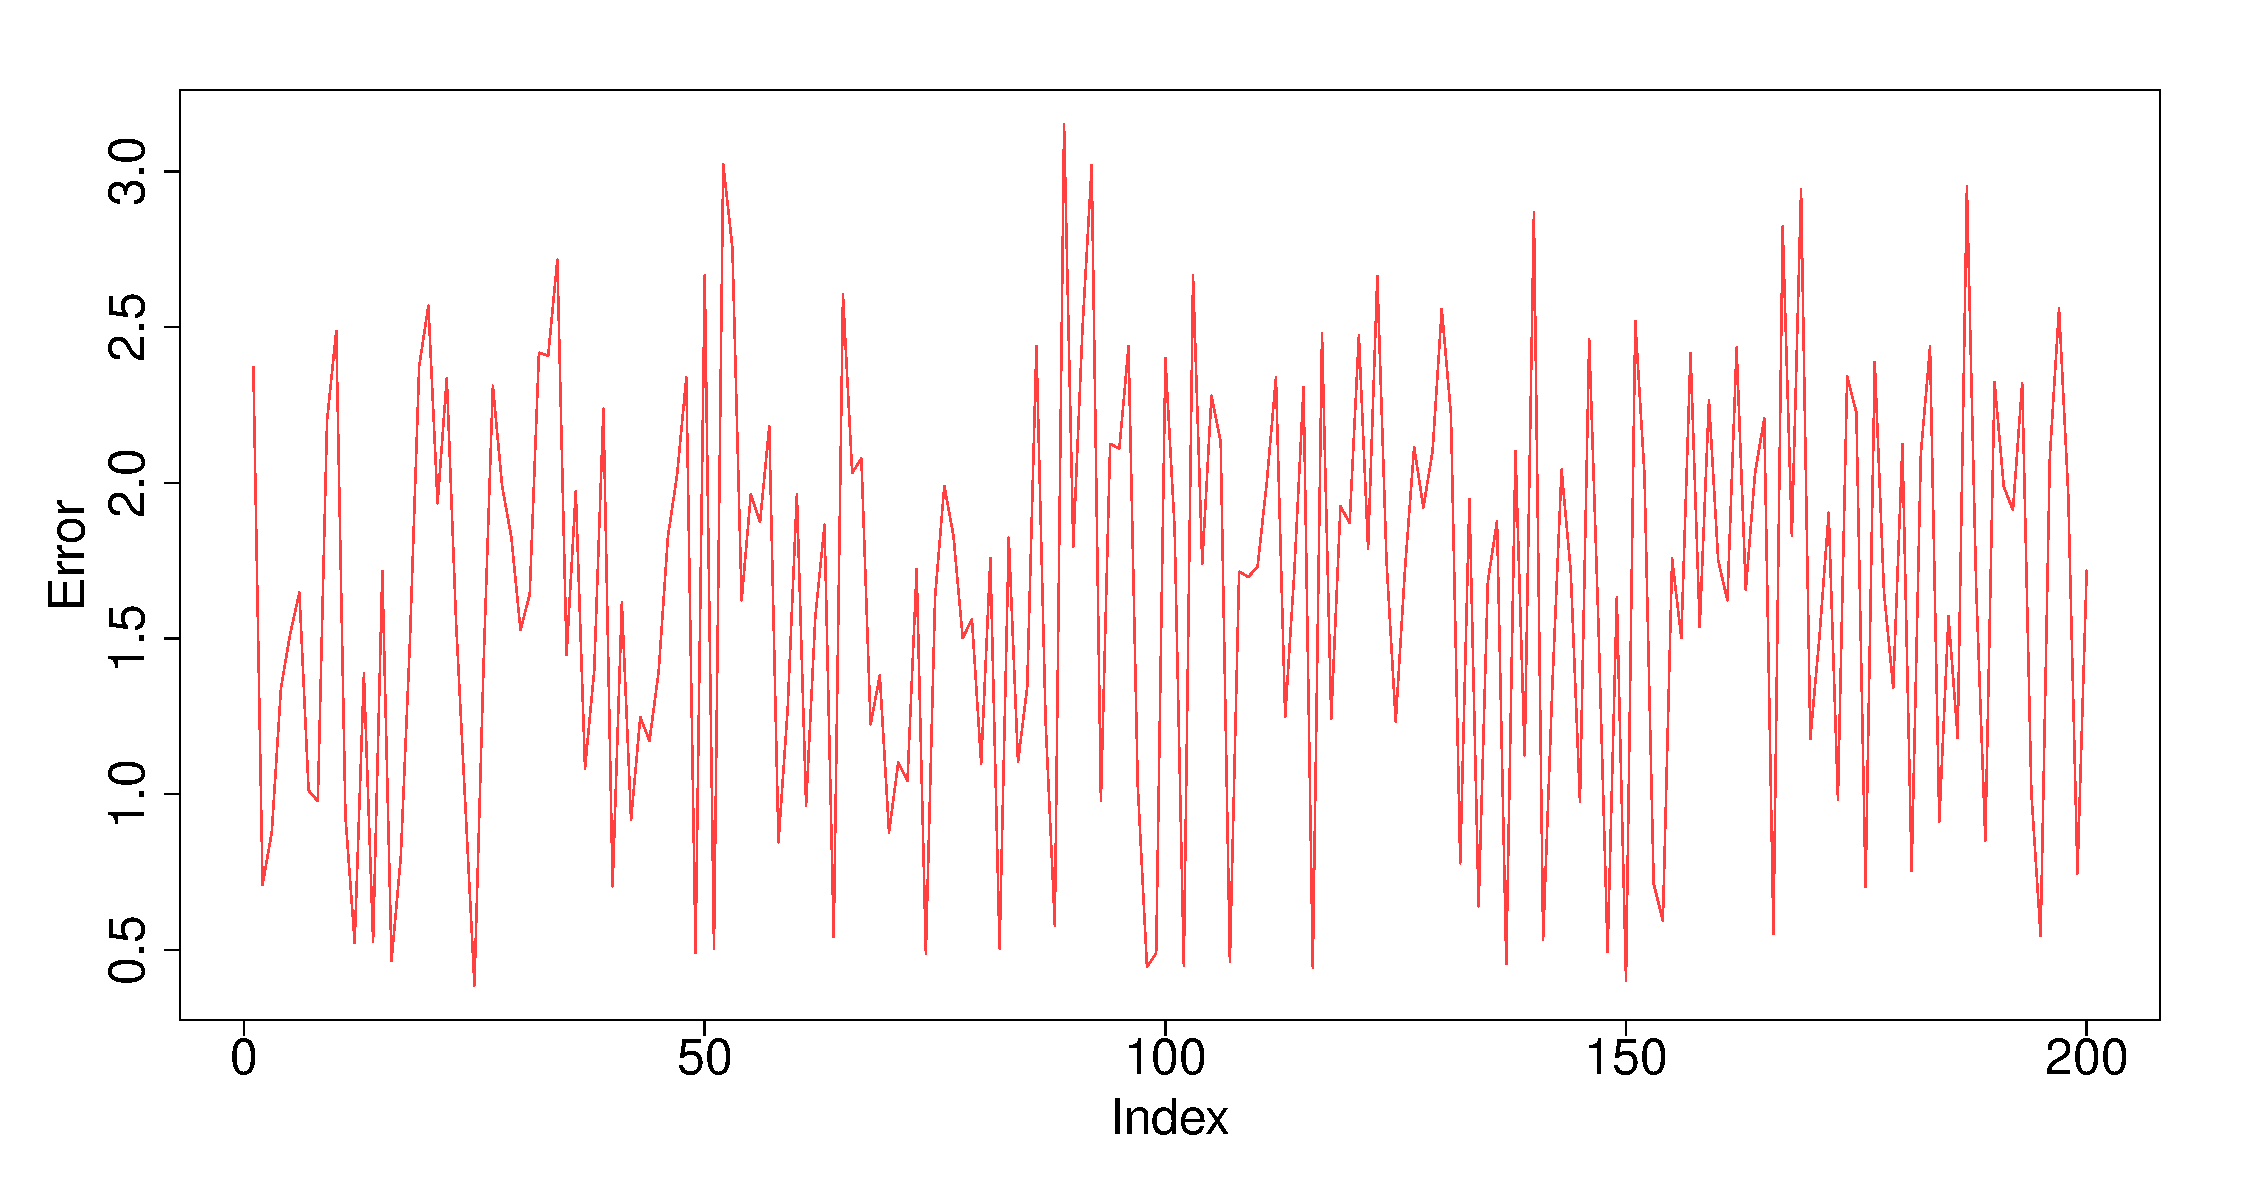
\includegraphics[width=\linewidth]{Figures/Pictures/TAA/Error_SK_AAPL2.pdf}
%         \caption{Error for $200$ points ATM.}
%     \label{Figures:APPL_Error}
%     \end{minipage}
%     \hfill
%     \begin{minipage}[t]{0.49\textwidth}
%         \centering
%         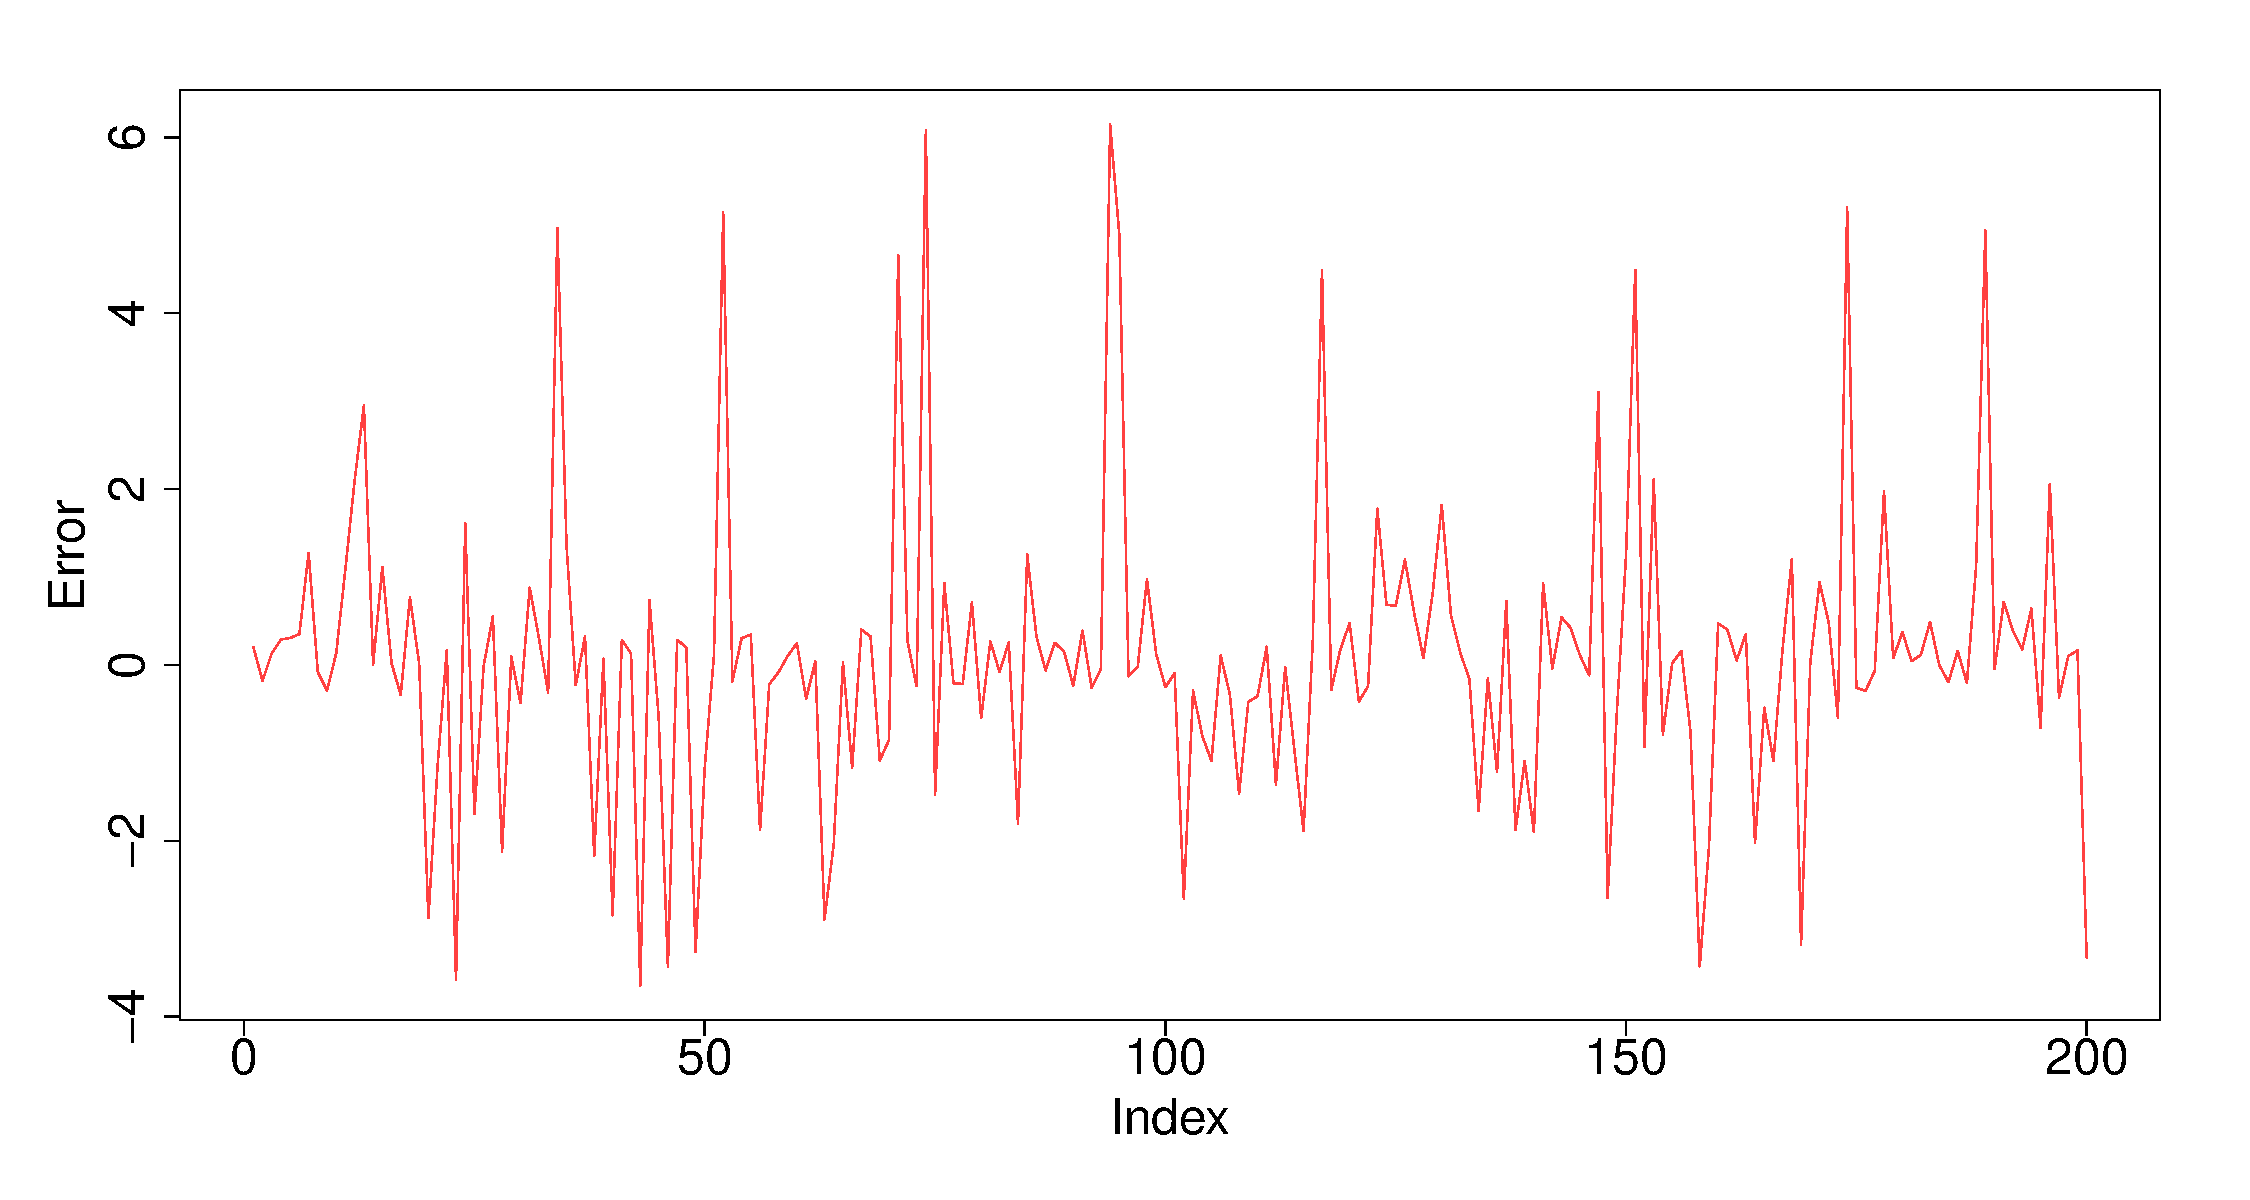
\includegraphics[width=\linewidth]{Figures/Pictures/TAA/Error_SK_AMZN2.pdf}
%         \caption{Error for $200$ points ATM.}
%     \label{Figures:AMZN_Error}
%     \end{minipage}
%     \begin{minipage}[t]{0.50\textwidth}
%         \centering
%         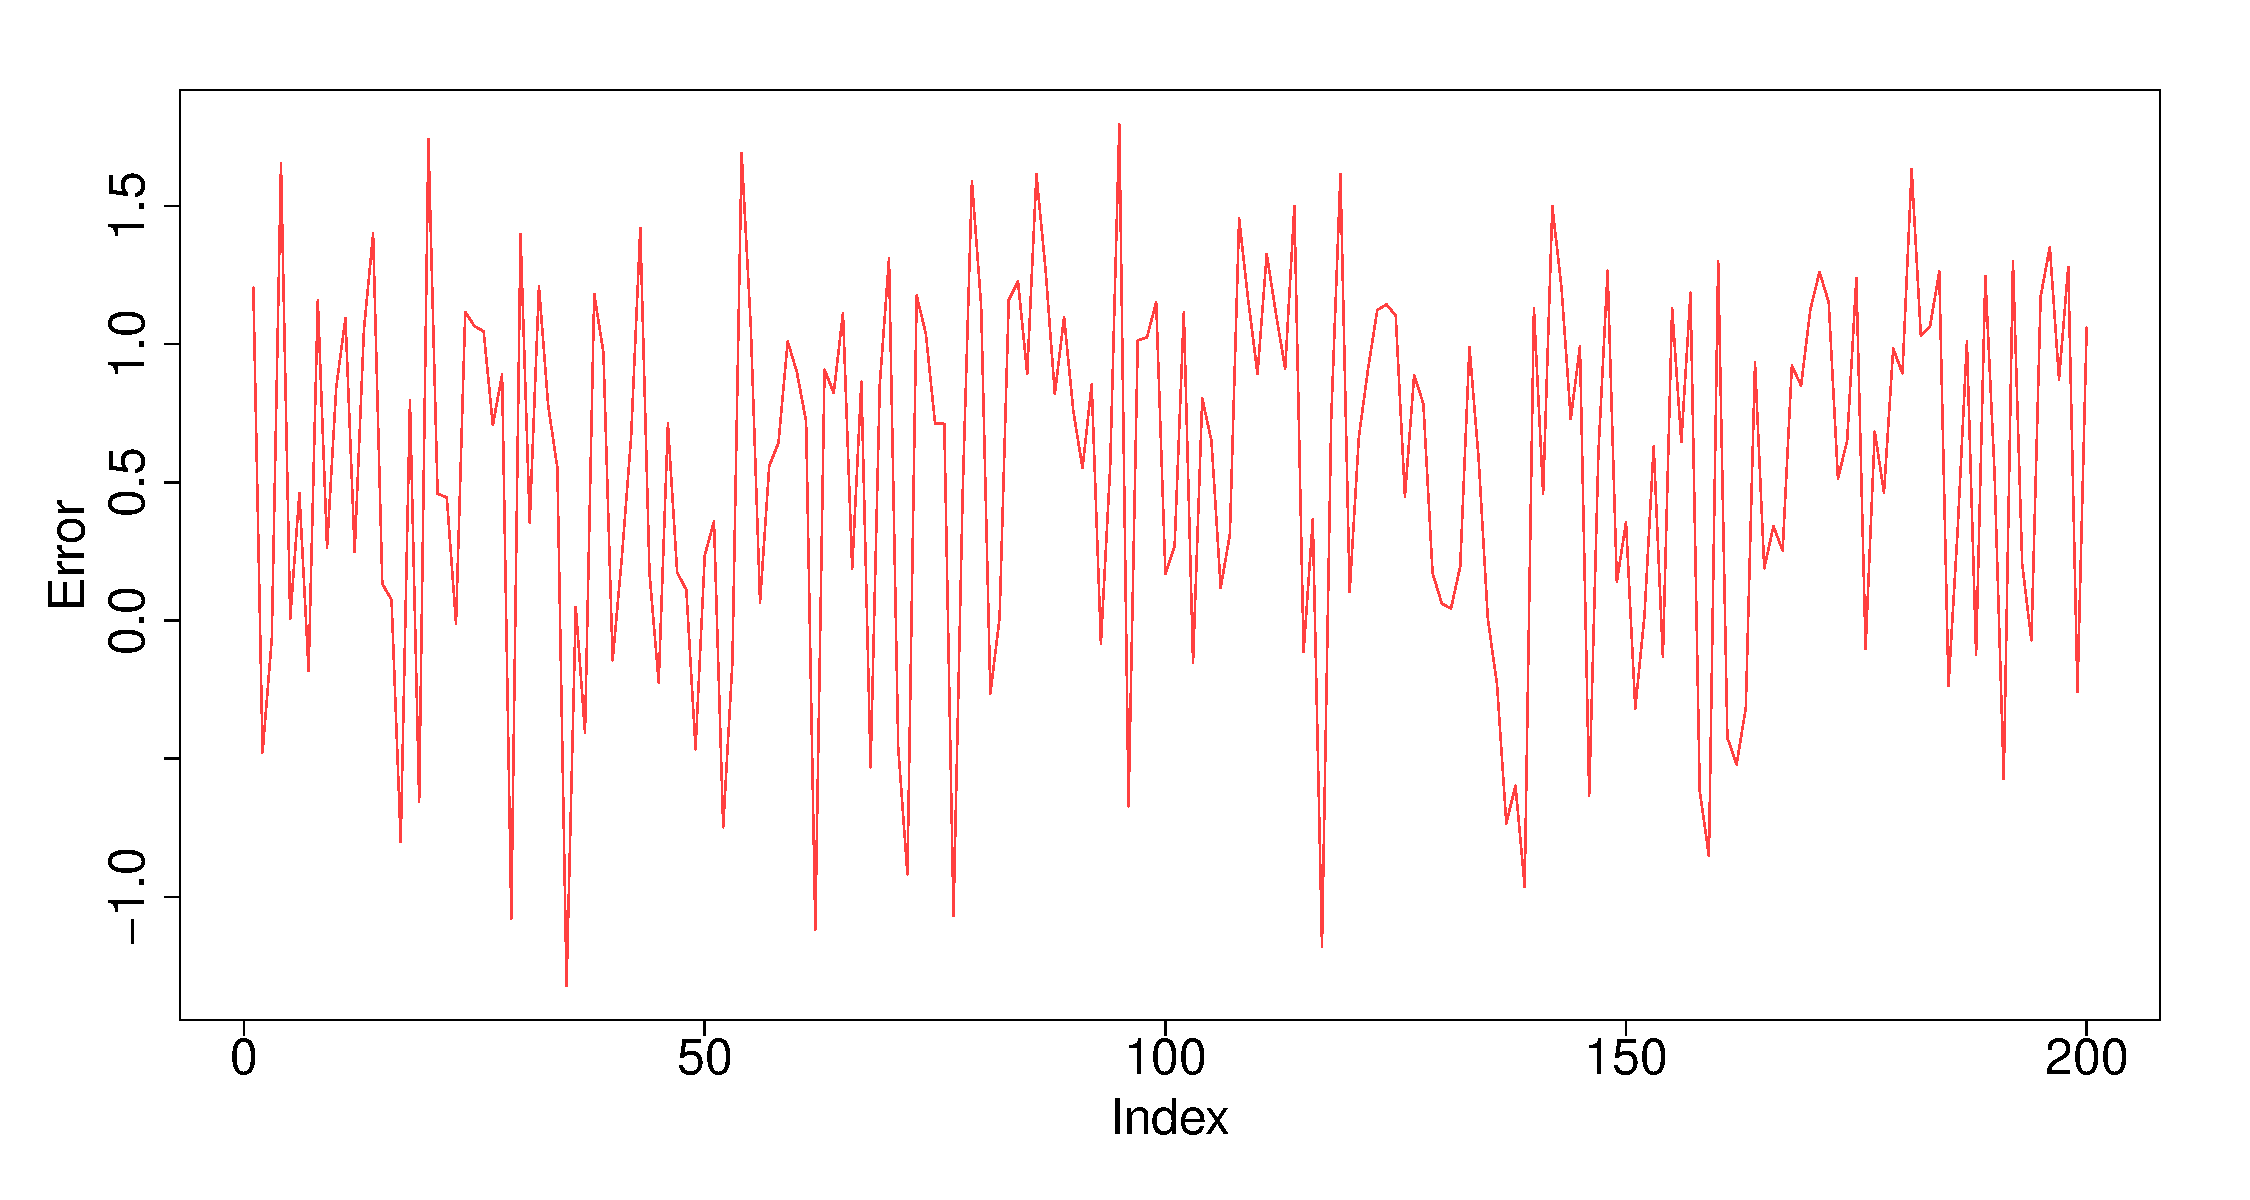
\includegraphics[width=\linewidth]{Figures/Pictures/TAA/Error_SK_TSLA2.pdf}
%         \caption{Error for $200$ points ATM.}
%     \label{Figures:TSLA_Error}
%     \end{minipage}
% \end{figure}

% As for GOOG we see a clear improvement of the error from the 200 random points to 200 points ATM. For the AAPL, AMZN and TSLA the error is $1.64$ ($35.06\%$), $0.08$ ($24.84\%$) and $0.54$ ($11.20\%$), respectively. Hence, comparing with GOOG all three stocks perform worse when looking ATM where we would expect the method to perform best. Furthermore, we see as expected that AMZN performs the worst comparing all four stocks. Again this could be explained by the volatility surface, both the one constructed by the data and the neural network, is not a smooth surface. This will also affect the derivatives of the implied volatility which is used to construct the risk-neutral density. Hence, this indicates that how the initial volatility surface look can affect the final results significantly. Furthermore, we have seen by comparing the results from GOOG, AAPL and TSLA that just because there are more point for network to train upon the results will not necessarily improve. However, this can very well also be because this network where specifically tuned to perfect the performance with respect to the data for GOOG. Lastly, we can conclude that this method, even ATM, still gives an error of 10 percent or more which is not optimal. This could be caused by using multiple approximation methods to get the final result, such as the neural network, the derivatives of this and the integral in \eqref{Eq:RND_Pricing}. All these point will be further discussed in \autoref{Ch.Discussion}. To address the problem with using a lot of approximation methods we will try to use neural networks to approximate the price function instead of the implied volatility surface. 

